\documentclass[15pt, mathserif]{beamer}

\usepackage[french]{babel}
\usepackage[T1]{fontenc}
\usepackage[utf8]{inputenc}
%\usepackage{esvect}
\usepackage{bm}
\usepackage{eurosym}
\usepackage{tikz}
\usepackage{pgf,tikz,pgfplots}
\pgfplotsset{compat=1.15}
\usepackage{mathrsfs}
\usetikzlibrary{arrows}
\usetikzlibrary{arrows.meta}

\usetikzlibrary{mindmap}
\usepackage{multicol}
\usepackage[tikz]{bclogo}
\usepackage{tkz-tab}
\usepackage{amsmath, tabu}
\usepackage{esvect} %\vv{AB} pour le vecteur AB

\DeclareMathOperator{\e}{e}

%% Tableau

\usepackage{makecell}
\setcellgapes{1pt}
\makegapedcells
\newcolumntype{R}[1]{>{\raggedleft\arraybackslash }b{#1}}
\newcolumntype{L}[1]{>{\raggedright\arraybackslash }b{#1}}
\newcolumntype{C}[1]{>{\centering\arraybackslash }b{#1}}


%pour avoir des parenthèses rondes dans le package fourier
\DeclareSymbolFont{cmoperators}   {OT1}{cmr} {m}{n}
\DeclareSymbolFont{cmlargesymbols}{OMX}{cmex}{m}{n}

\usefonttheme{professionalfonts} %permet d'enlever un bug avec fourier
\usepackage{fourier}
\DeclareMathDelimiter{(}{\mathopen} {cmoperators}{"28}{cmlargesymbols}{"00}
\DeclareMathDelimiter{)}{\mathclose}{cmoperators}{"29}{cmlargesymbols}{"01}

%Graphiques 

\usepackage{pgf,tikz,pgfplots}
\pgfplotsset{compat=1.15}
\usepackage{mathrsfs}
\usetikzlibrary{arrows}
\usetikzlibrary{mindmap}

%ensembles de nbres

\newcommand{\R}{\mathbb{R}}			%permet d'écrire le R "ensemble des réels"'
\newcommand{\N}{\mathbb{N}}			%permet d'écrire le N "ensemble des entiers naturels"
\newcommand{\Z}{\mathbb{Z}}			%permet d'écrire le Z "ensemble des entiers relatifs"
\newcommand{\Prem}{\mathbb{P}}	%permet d'écrire le P "ensemble des nombres premiers" (qui n'a pas marché avec le \P car il existe déjà)
\newcommand{\D}{\mathbb{D}}
\newcommand{\Df}{\mathcal{D}_f}
\newcommand{\Cf}{\mathcal{C}_f}

\newcommand{\Q}{\mathbb{Q}}


\newcommand{\st}[1]{$(#1_n)_{n \in \N}$}

\usetheme{Madrid}
\useoutertheme{miniframes} % Alternatively: miniframes, infolines, split
\useinnertheme{circles}
\definecolor{UBCblue}{rgb}{0.1, 0.25, 0.4} % UBC Blue (primary)
\definecolor{bordeaux}{RGB}{128,0,0}
\usecolortheme[named=UBCblue]{structure}

\usepackage{color} % J'aime bien définir mes couleurs
\definecolor{propcolor}{rgb}{0, 0.5, 1}
\definecolor{thcolor}{rgb}{0.6, 0.07, 0.07}
\colorlet{louis}{blue!70!green!60!white}
\colorlet{sakura}{pink!40!red}

\title{Activités Mentales}
\date{24 Août 2023}

\newcommand{\vco}[2]{\begin{pmatrix} #1 \\ #2 \end{pmatrix}} %Coordonnées de vecteur
\newenvironment{eq}{\begin{cases}\begin{tabu}{ccccc}}{\end{tabu}\end{cases}}
\newenvironment{eql}{\begin{cases}\begin{tabu}{cccccl}}{\end{tabu}\end{cases}}
\newenvironment{eqrl}{\begin{cases}\begin{tabu}{rl}}{\end{tabu}\end{cases}}

\newenvironment{Eq}{\begin{center}\begin{tabular}{rrcl}}{\end{tabular}\end{center}}
\newcommand{\ligneq}[2]{$\Longleftrightarrow$ & $#1$ & $=$ & $#2$ \\}
\newcommand{\Ligneq}[2]{ & $#1$ & $=$ & $#2$ \\}

\newenvironment{RPN}{\begin{center}\begin{tabular}{rrclcrcl}}{\end{tabular}\end{center}}
\newcommand{\Lignerpn}[4]{ & $#1$ & $=$ & $#2$ & ou & $#3$ & $=$ & $#4$ \\}
\newcommand{\lignerpn}[4]{$\Longleftrightarrow$ & $#1$ & $=$ & $#2$ & ou & $#3$ & $=$ & $#4$ \\}

\newenvironment{TRPN}{\begin{center}\begin{tabular}{rrclcrclcrcl}}{\end{tabular}\end{center}}
\newcommand{\Lignetrpn}[6]{ & $#1$ & $=$ & $#2$ & ou & $#3$ & $=$ & $#4$ & ou & $#5$ & $=$ & $#6$ \\}
\newcommand{\lignetrpn}[6]{$\Longleftrightarrow$ & $#1$ & $=$ & $#2$ & ou & $#3$ & $=$ & $#4$ & ou & $#5$ & $=$ & $#6$ \\}
\begin{document}

\begin{frame}
    \titlepage
\end{frame}

\begin{frame} 
	\frametitle{Question 1}
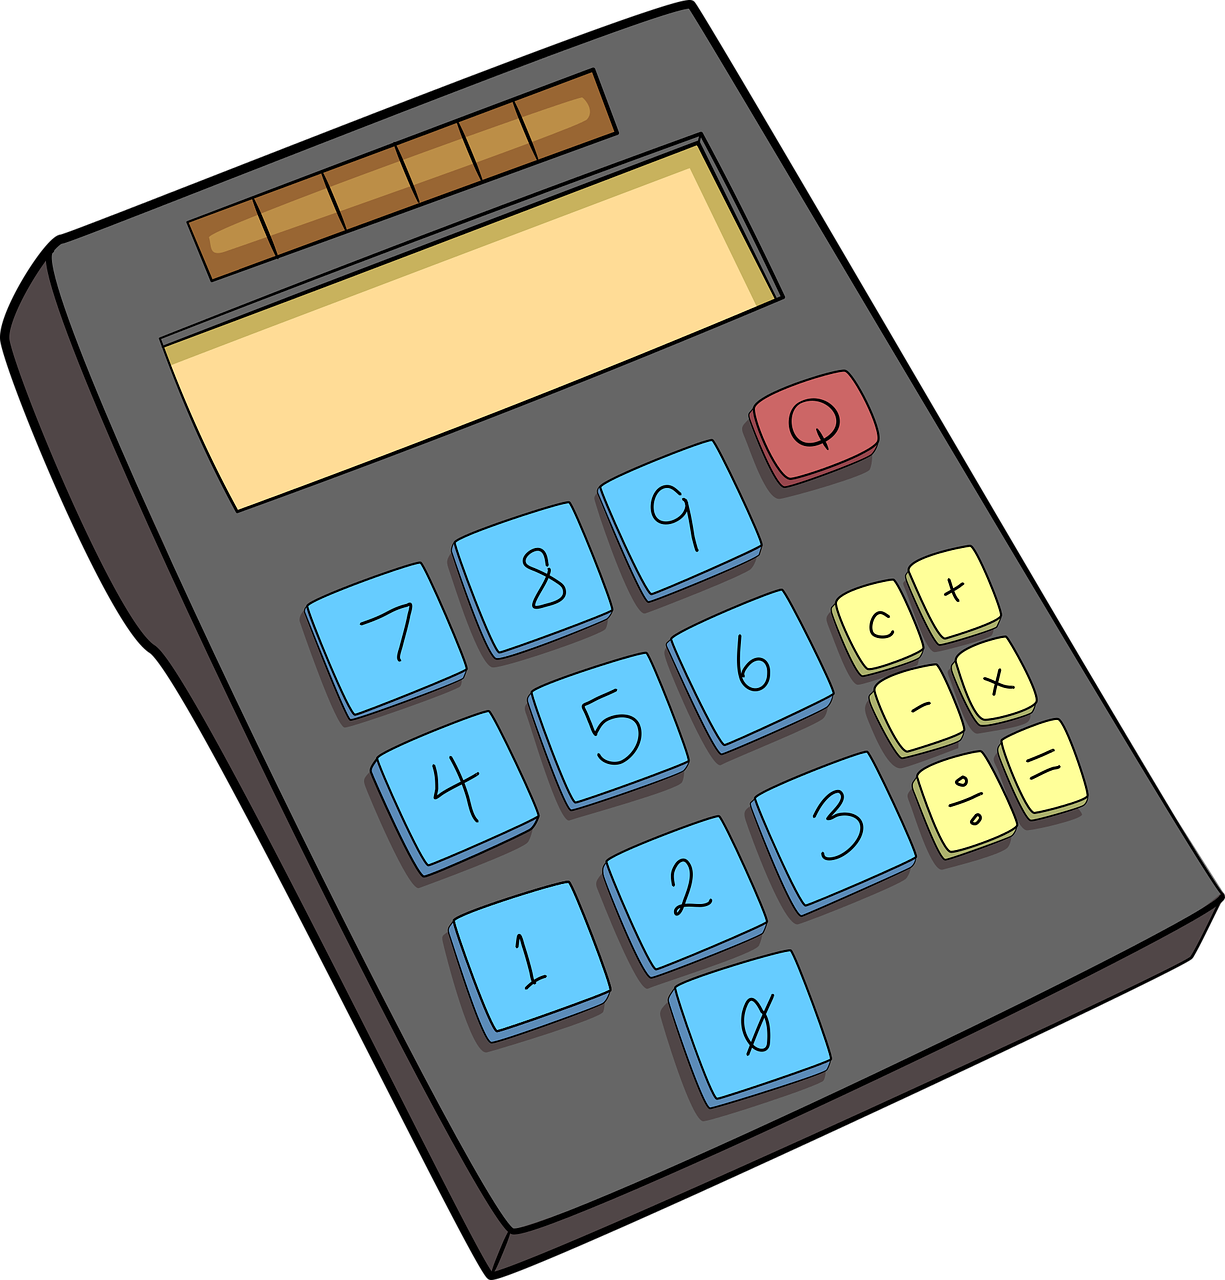
\includegraphics[scale=0.01]{calculatrice} Un article diminue de 34\% puis de 80\%. Quelle est l'évolution globale ?\end{frame}


\begin{frame} 
	\frametitle{Question 2}
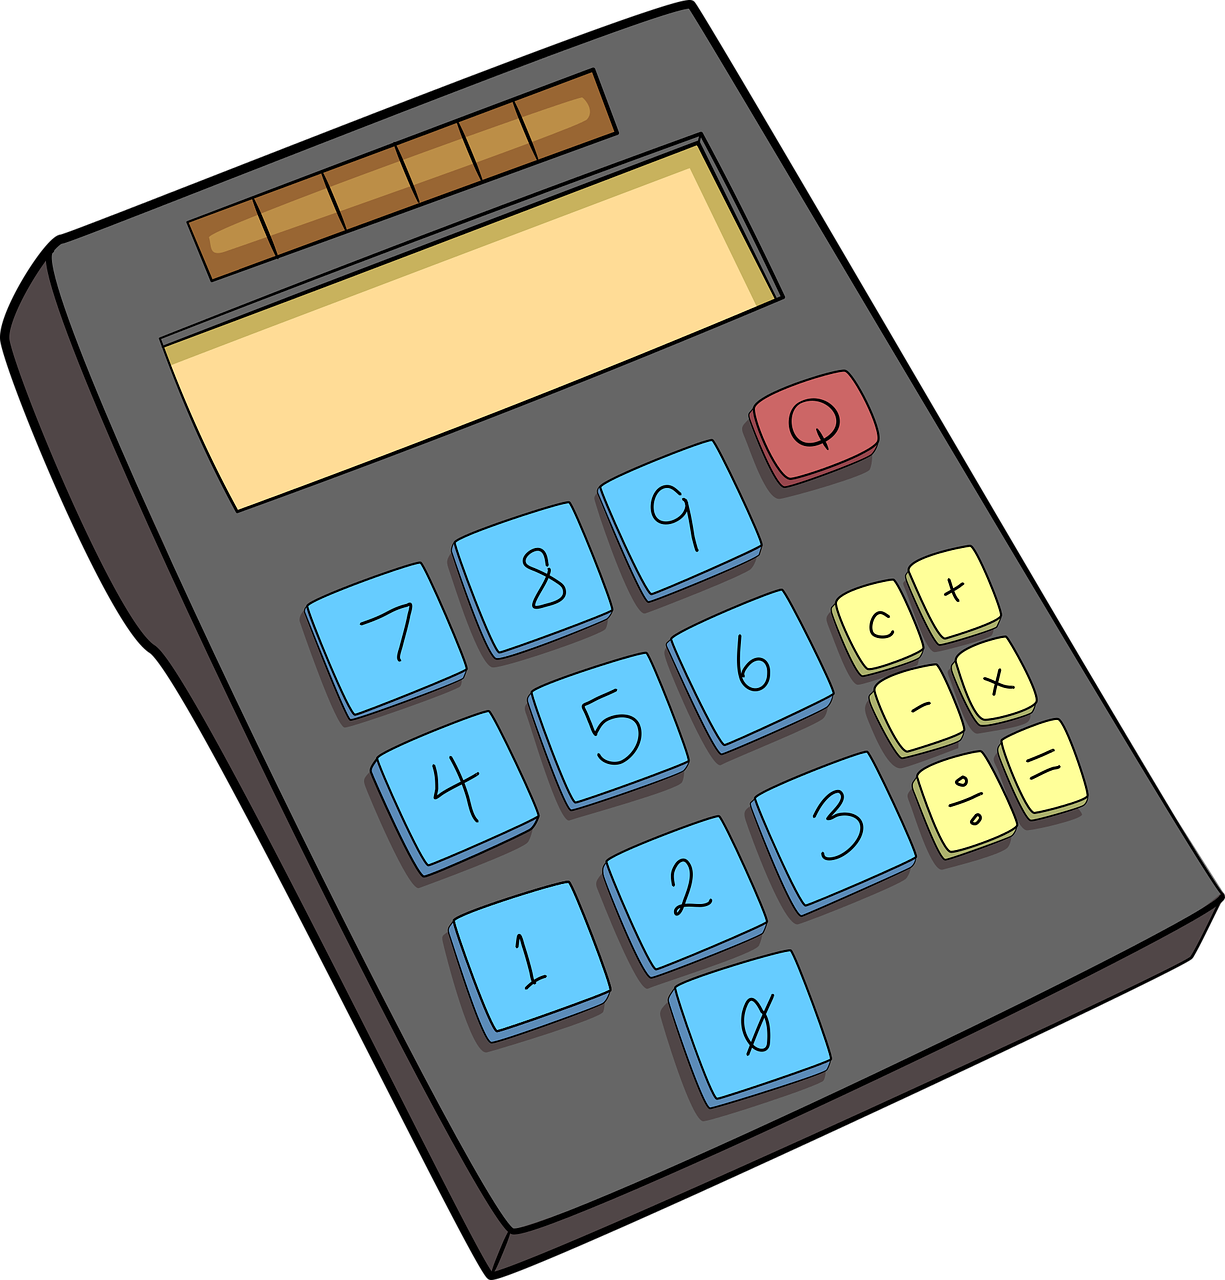
\includegraphics[scale=0.01]{calculatrice} Un article augmente de 46\% puis diminue de 83\%. Quelle est l'évolution globale ?\end{frame}


\begin{frame} 
	\frametitle{Question 3}
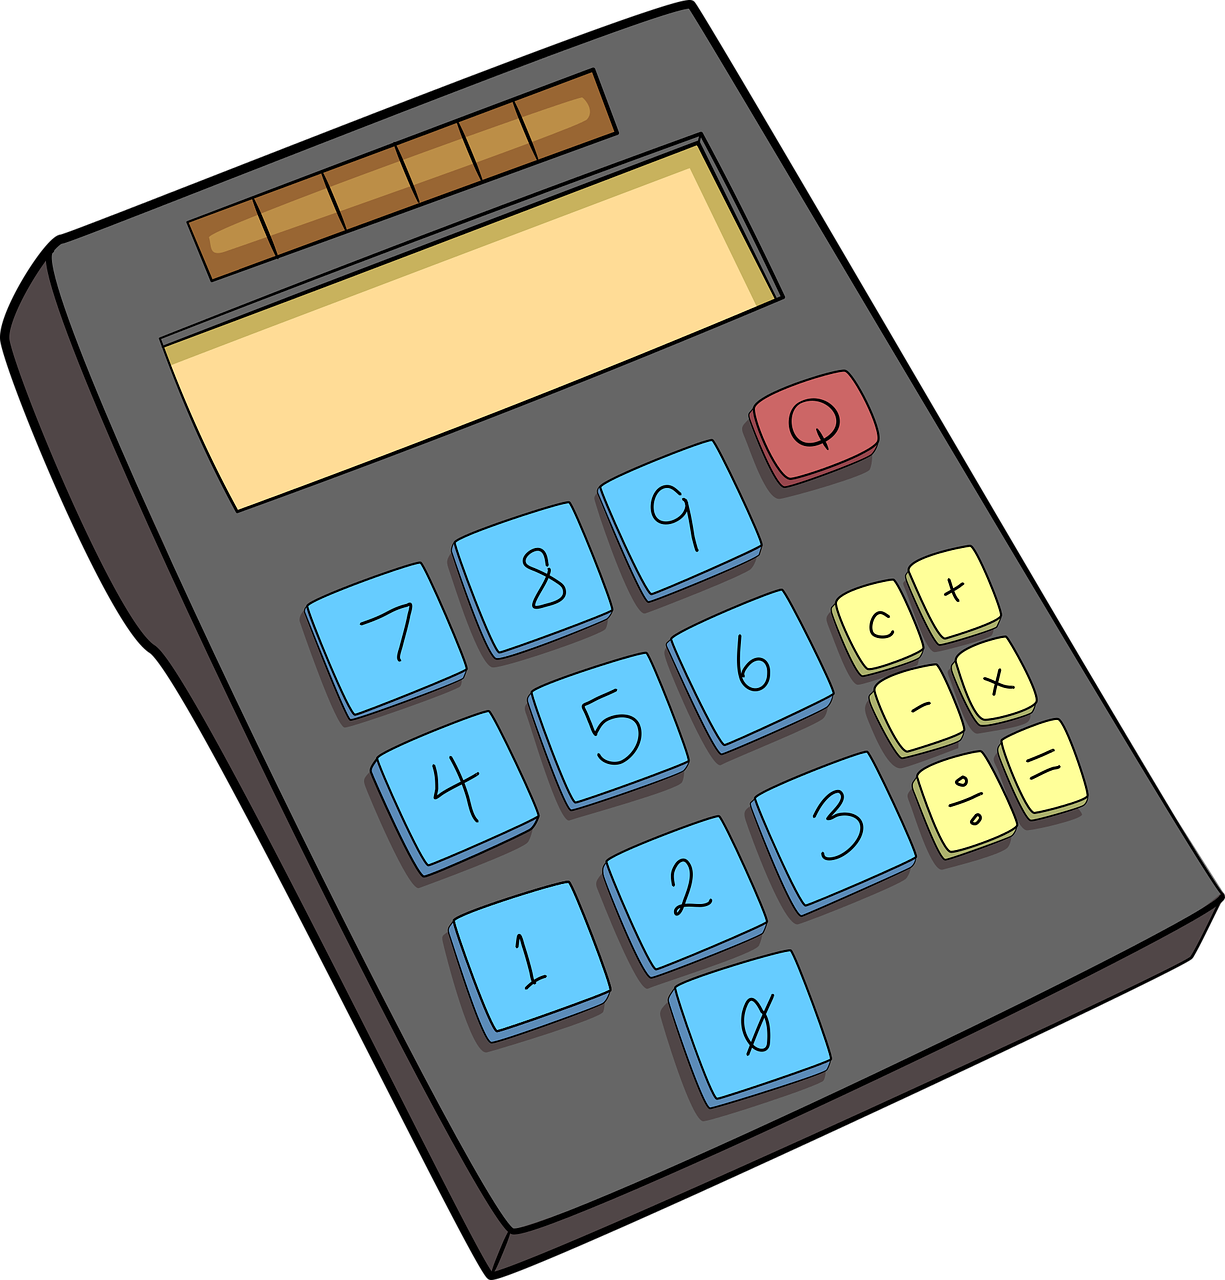
\includegraphics[scale=0.01]{calculatrice} Un article augmente de 48\% puis de 60\%. Quelle est l'évolution globale ?\end{frame}


\begin{frame} 
	\frametitle{Question 4}
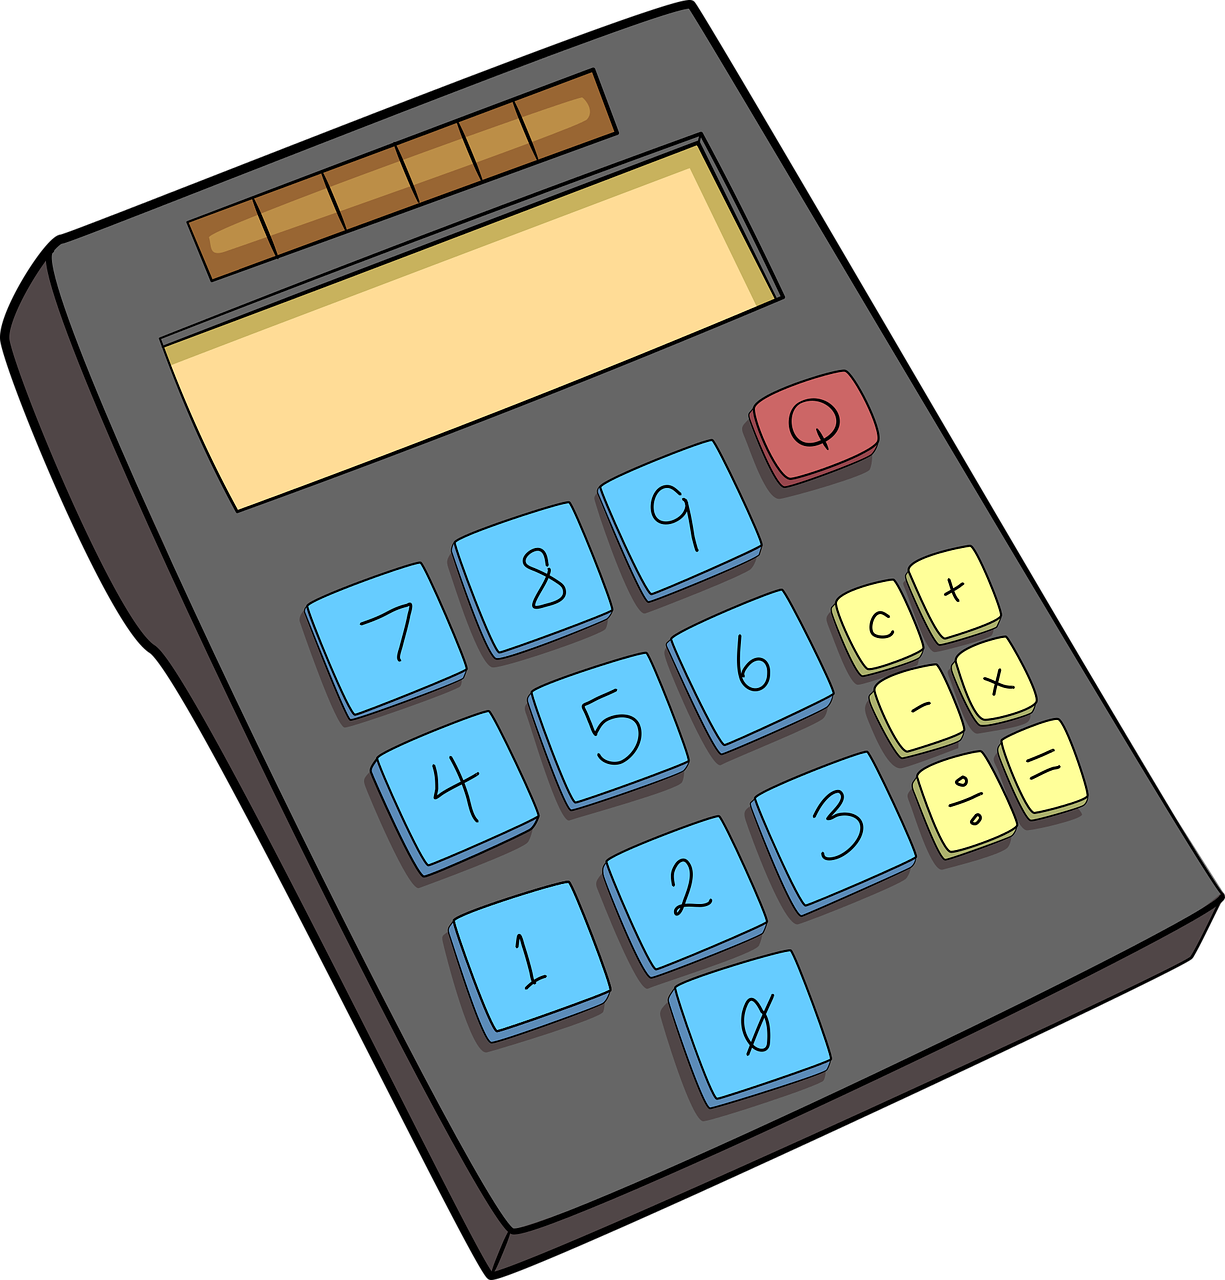
\includegraphics[scale=0.01]{calculatrice} Un article diminue de 53\% puis de 3\%. Quelle est l'évolution globale ?\end{frame}


\begin{frame} 
	\frametitle{Question 5}
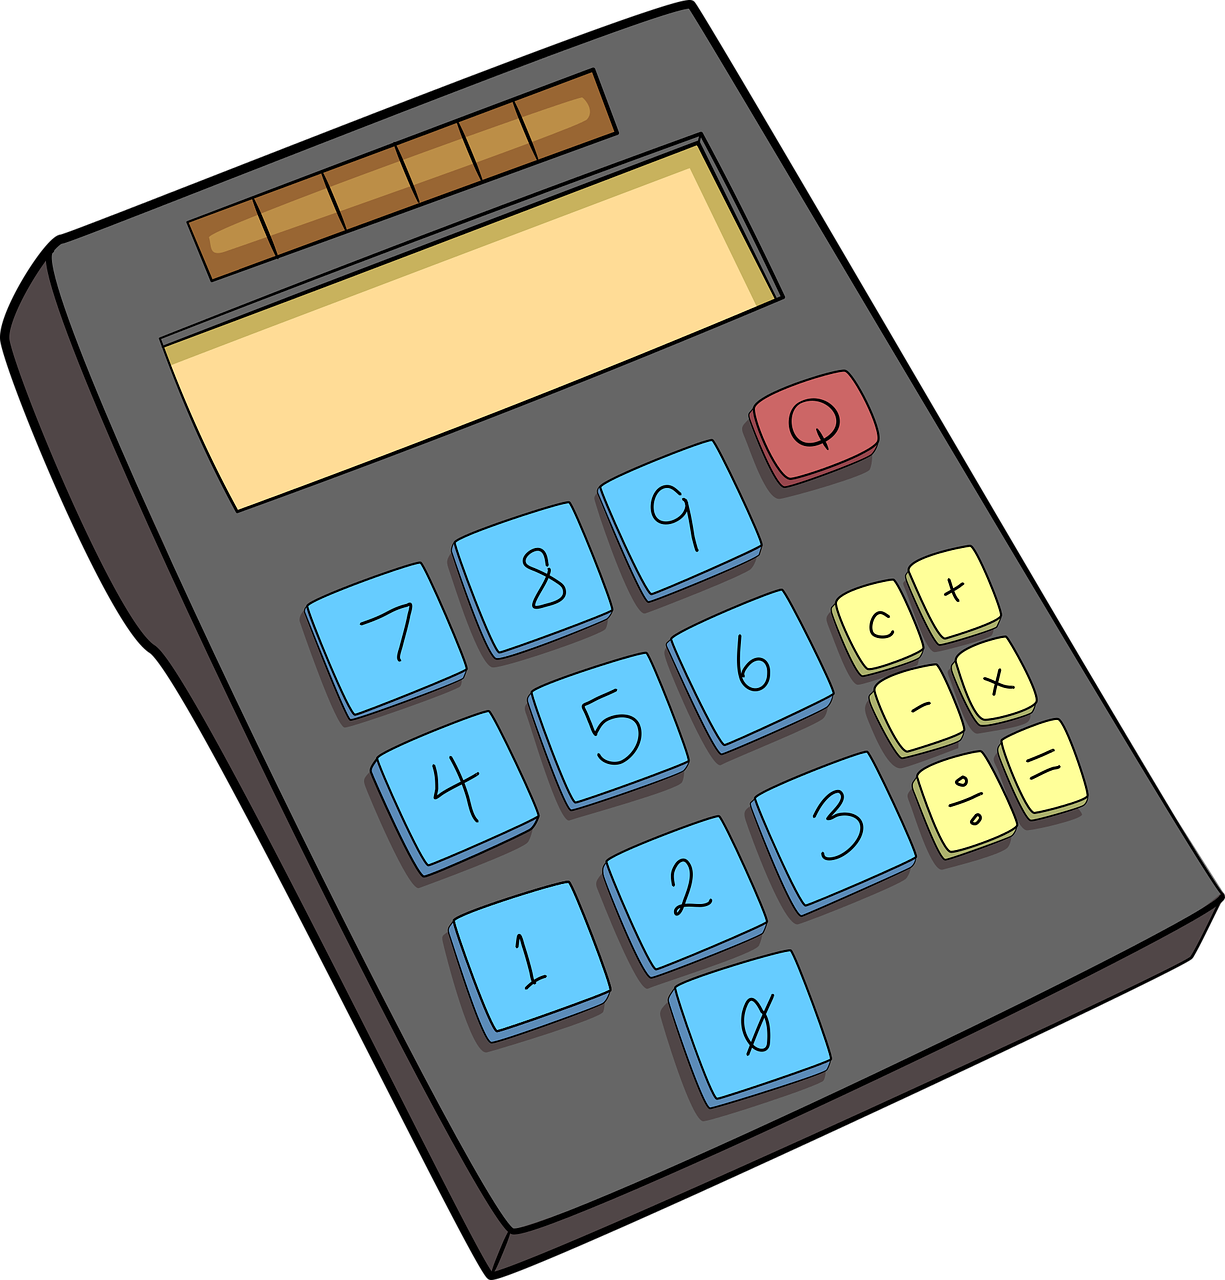
\includegraphics[scale=0.01]{calculatrice} Un article augmente de 5\% puis de 93\%. Quelle est l'évolution globale ?\end{frame}


\begin{frame}
\vspace{-10mm}
	\frametitle{Correction 1}
\vspace*{1cm} Un article diminue de 34\% puis de 80\%. Quelle est l'évolution globale ? \\ Le coefficient multiplicateur associé à une diminution de 34\% est $1-\dfrac{34}{100} = 0.66$ et le coefficient multiplicateur associé à une diminution de 80\% est $1-\dfrac{80}{100} = 0.2$. Pour connaitre l'évolution globale, on multiplie les deux coefficients multiplicateurs, on a $ 0.66 \times 0.2=0.13$. On cherche alors quelle évolution est associée à ce coefficient multiplicateur : $0.13-1 =-0.87$. Ainsi l'évolution globale est une diminution de 86.8\%. 
 \begin{center} 
 \begin{tikzpicture} 
 \node[draw] (P) at (0,0) {{\small Prix initial}}; 
 \node[draw] (S) at (4,0) {{\small Prix intermédiaire}}; 
 \node[draw] (T) at (8,0) {{\small Prix final}};
 \draw[->,>=latex] (P) to[bend left=20]  node[midway,above] {{\small 0.66}} (S) ; 
 \draw[->,>=latex] (S) to[bend left=20]  node[midway,above] {{\small 0.2}} (T) ; 
 \draw[->,>=latex] (P) to[bend right=20]  node[midway,below] {{\small0.13}} (T) ; 
 \end{tikzpicture} 
 \end{center}\end{frame}


\begin{frame}
\vspace{-10mm}
	\frametitle{Correction 2}
\vspace*{1cm} Un article augmente de 46\% puis diminue de 83\%. Quelle est l'évolution globale ? \\ Le coefficient multiplicateur associé à une augmentation de 46\% est $1+\dfrac{46}{100} = 1.46$ et le coefficient multiplicateur associé à une diminution d'environ' 83\% est $1-\dfrac{83}{100} = 0.17$. Pour connaitre l'évolution globale, on multiplie les deux coefficients multiplicateurs, on a $ 1.46 \times 0.17=0.25$. On cherche alors quelle évolution est associée à ce coefficient multiplicateur : $0.25-1 =-0.75$. Ainsi l'évolution globale est une diminution d'environ 75.0\%. 
 \begin{center} 
 \begin{tikzpicture} 
 \node[draw] (P) at (0,0) {{\small Prix initial}}; 
 \node[draw] (S) at (4,0) {{\small Prix intermédiaire}}; 
 \node[draw] (T) at (8,0) {{\small Prix final}};
 \draw[->,>=latex] (P) to[bend left=20]  node[midway,above] {{\small 1.46}} (S) ; 
 \draw[->,>=latex] (S) to[bend left=20]  node[midway,above] {{\small 0.17}} (T) ; 
 \draw[->,>=latex] (P) to[bend right=20]  node[midway,below] {{\small0.25}} (T) ; 
 \end{tikzpicture} 
 \end{center}\end{frame}


\begin{frame}
\vspace{-10mm}
	\frametitle{Correction 3}
\vspace*{1cm} Un article augmente de 48\% puis de 60\%. Quelle est l'évolution globale ? \\ Le coefficient multiplicateur associé à une augmentation de 48\% est $1+\dfrac{48}{100} = 1.48$ et le coefficient multiplicateur associé à une augmentation de 60\% est $1+\dfrac{60}{100} = 1.6$. Pour connaitre l'évolution globale, on multiplie les deux coefficients multiplicateurs, on a $ 1.48 \times 1.6=2.37$. On cherche alors quelle évolution est associée à ce coefficient multiplicateur : $2.37-1 =1.37$. Ainsi l'évolution globale est d'environ 137.0\%. 
 \begin{center} 
 \begin{tikzpicture} 
 \node[draw] (P) at (0,0) {{\small Prix initial}}; 
 \node[draw] (S) at (4,0) {{\small Prix intermédiaire}}; 
 \node[draw] (T) at (8,0) {{\small Prix final}};
 \draw[->,>=latex] (P) to[bend left=20]  node[midway,above] {{\small $ \times1.48$}} (S) ; 
 \draw[->,>=latex] (S) to[bend left=20]  node[midway,above] {{\small $\times 1.6$}} (T) ; 
 \draw[->,>=latex] (P) to[bend right=20]  node[midway,below] {{\small $\times 2.37$}} (T) ; 
 \end{tikzpicture} 
 \end{center}\end{frame}


\begin{frame}
\vspace{-10mm}
	\frametitle{Correction 4}
\vspace*{1cm} Un article diminue de 53\% puis de 3\%. Quelle est l'évolution globale ? \\ Le coefficient multiplicateur associé à une diminution de 53\% est $1-\dfrac{53}{100} = 0.47$ et le coefficient multiplicateur associé à une diminution de 3\% est $1-\dfrac{3}{100} = 0.97$. Pour connaitre l'évolution globale, on multiplie les deux coefficients multiplicateurs, on a $ 0.47 \times 0.97=0.46$. On cherche alors quelle évolution est associée à ce coefficient multiplicateur : $0.46-1 =-0.54$. Ainsi l'évolution globale est une diminution de 54.41\%. 
 \begin{center} 
 \begin{tikzpicture} 
 \node[draw] (P) at (0,0) {{\small Prix initial}}; 
 \node[draw] (S) at (4,0) {{\small Prix intermédiaire}}; 
 \node[draw] (T) at (8,0) {{\small Prix final}};
 \draw[->,>=latex] (P) to[bend left=20]  node[midway,above] {{\small 0.47}} (S) ; 
 \draw[->,>=latex] (S) to[bend left=20]  node[midway,above] {{\small 0.97}} (T) ; 
 \draw[->,>=latex] (P) to[bend right=20]  node[midway,below] {{\small0.46}} (T) ; 
 \end{tikzpicture} 
 \end{center}\end{frame}


\begin{frame}
\vspace{-10mm}
	\frametitle{Correction 5}
\vspace*{1cm} Un article augmente de 5\% puis de 93\%. Quelle est l'évolution globale ? \\ Le coefficient multiplicateur associé à une augmentation de 5\% est $1+\dfrac{5}{100} = 1.05$ et le coefficient multiplicateur associé à une augmentation de 93\% est $1+\dfrac{93}{100} = 1.93$. Pour connaitre l'évolution globale, on multiplie les deux coefficients multiplicateurs, on a $ 1.05 \times 1.93=2.03$. On cherche alors quelle évolution est associée à ce coefficient multiplicateur : $2.03-1 =1.03$. Ainsi l'évolution globale est d'environ 103.0\%. 
 \begin{center} 
 \begin{tikzpicture} 
 \node[draw] (P) at (0,0) {{\small Prix initial}}; 
 \node[draw] (S) at (4,0) {{\small Prix intermédiaire}}; 
 \node[draw] (T) at (8,0) {{\small Prix final}};
 \draw[->,>=latex] (P) to[bend left=20]  node[midway,above] {{\small $ \times1.05$}} (S) ; 
 \draw[->,>=latex] (S) to[bend left=20]  node[midway,above] {{\small $\times 1.93$}} (T) ; 
 \draw[->,>=latex] (P) to[bend right=20]  node[midway,below] {{\small $\times 2.03$}} (T) ; 
 \end{tikzpicture} 
 \end{center}\end{frame}




\end{document}